\section{问题二的模型的建立和求解}
\subsection{问题二的描述与分析}

问题二考虑动态环境下的多时间段资源分配场景。与问题一的静态单时刻分配不同,问题二面临用户移动性、信道时变性以及任务队列动态变化的复杂问题。在 $T_{\mathrm{tot}}$ 的观测窗口内,系统需要每 $T_w$ 进行一次资源分配决策,既要处理新到达的任务,又要考虑积压在排队队列中的历史任务。这是一个多阶段动态优化问题,需要在时间维度上综合考虑任务到达、信道变化和排队延迟的耦合影响\upcite{ZGDC201617011}。

\subsection{预备工作}

\subsubsection{模型预测控制(MPC)简介}

模型预测控制(Model Predictive Control, MPC)是一种先进的控制策略,广泛应用于工业控制、自动驾驶、机器人等领域。它通过预测未来系统的行为,优化当前的控制输入,从而实现对复杂系统的高效控制\upcite{TYLX202406019}。

\textbf{核心思想:}

\textbf{基于模型的预测:}
MPC利用系统的数学模型(如状态空间模型、传递函数等)预测未来一段时间内系统的输出行为\upcite{ZGXJ202411011}。

\textbf{滚动优化:}
在每个时刻,MPC通过求解一个优化问题,找到未来一段时间的最优控制输入序列,使系统输出尽可能接近目标,同时满足约束条件。

\textbf{反馈调整:}
只执行当前时刻的控制输入,随后根据新的测量值更新预测,重复上述过程。这种滚动优化和反馈机制使MPC能够应对系统的不确定性和扰动。
\subsection{模型建立}

问题二模型大部分与问题一相同,可直接复用问题一中的模型,不再重复说明。不同之处在于问题二允许 $t$ 在决策窗口内按 $\mathcal{T}=\{0,100,\dots,900\}$ 演化,并引入任务到达与队列动态,下面将具体阐述。
\subsubsection{任务队列动态演化模型}

为精确描述任务的动态变化,我们引入两个时间尺度:
\begin{itemize}
    \item \textbf{决策时刻 $t$}:每100ms进行一次资源分配决策,对应$t \in \{0, 100, 200, \ldots, 900\}$。
    \item \textbf{仿真时刻 $\tau$}:以1ms为步长,用于模拟任务到达和信道变化,$\tau$表示具体的毫秒时刻。
\end{itemize}

定义用户$k$在时刻$t$的任务队列状态:

\begin{itemize}
  \item $A_{k,\tau}(t)$:用户$k$在时刻$\tau$到达且在时刻$t$仍在队列中的任务数据量
  \item $Q_k(t) = \sum_{\tau=0}^{t} A_{k,\tau}(t)$:用户$k$在时刻$t$的总排队任务量
\end{itemize}

任务队列的动态演化遵循以下规律:

\textbf{(1) 任务到达:}
在每个1ms时刻$\tau$,根据数据文件读取新到达任务:
\begin{equation}
A_{k,\tau}(\tau) = \text{TaskFlow}_k(\tau)
\end{equation}

\textbf{(2) 任务服务:}
在决策时刻$t$,若用户$k$被分配$i_k(t)$个RB,则在接下来的100ms内可传输的数据量为:
\begin{equation}
S_k(t) = r_k(t) \times 0.1 \times 10^{-6} 
\end{equation}

\textbf{(3) 队列更新:}
任务按FIFO(先进先出)顺序服务,队列更新规则为:
\begin{equation}
\label{eq:queue_evolution}
Q_k(t+100) = \max\left(0, Q_k(t) + \sum_{\tau=t+1}^{t+100} \text{TaskFlow}_k(\tau) - S_k(t)\right)
\end{equation}

\subsubsection{时延计算模型(任务级)}
 
由于存在到达过程,问题二按任务到达时刻进行时延度量。对于用户$k$在时刻$\tau$到达的任务,其总时延包含排队时延和传输时延:

\textbf{(1) 排队时延:}
任务在时刻$\tau$到达,在时刻$t_{\text{start}}$开始服务,则排队时延为:
\begin{equation}
Q_{k,\tau} = t_{\text{start}} - \tau
\end{equation}

\textbf{(2) 传输时延:}
假设任务从时刻$t_{\text{start}}$开始传输,数据量为$D_{k,\tau}$,则传输时延为:
\begin{equation}
T_{k,\tau} = \frac{D_{k,\tau} \times 10^6}{r_k(t_{\text{start}})}
\end{equation}

\textbf{(3) 总时延:}
\begin{equation}
L_{k,\tau}^s = Q_{k,\tau} + T_{k,\tau}, \quad s \in \{U, e, m\}
\end{equation}


\subsubsection{窗口内 QoS 计分规则}
仅对“\textbf{在当前窗口内完成}”的 URLLC/eMBB 任务计分;mMTC 采用“\textbf{本窗到达用户的比例计分}”。令窗口 $t$ 的结束时刻为 $t+100$,定义集合:
\begin{align}
\mathcal{F}_U(t) &= \big\{(k,\tau_0)\mid k\in\mathcal{U}_U,\; \tau_f\in[t,\,t+T_w)\big\}, \\
\mathcal{F}_e(t) &= \big\{(k,\tau_0)\mid k\in\mathcal{U}_e,\; \tau_f\in[t,\,t+T_w)\big\}.
\end{align}

\begin{align}
Y_U(t) &= \sum_{(k,\tau_0)\in\mathcal{F}_U(t)} y_{k,\tau_0}^U, 
\quad y_{k,\tau_0}^U =\begin{cases}
\alpha^{L_{k,\tau_0}} & \text{若 } L_{k,\tau_0}\le L_U^{\text{SLA}} \\
-M_U & \text{若 } L_{k,\tau_0}> L_U^{\text{SLA}}
\end{cases}
\end{align}

\begin{align}
Y_e(t) &= \sum_{(k,\tau_0)\in\mathcal{F}_e(t)} y_{k,\tau_0}^e, 
\quad y_{k,\tau_0}^e =\begin{cases}
1 & \text{若 } L_{k,\tau_0}\le L_e^{\text{SLA}} \text{ 且 } r_{\mathrm{avg}}\ge r_e^{\text{SLA}} \\
\dfrac{r_{\mathrm{avg}}}{r_e^{\text{SLA}}} & \text{若 } L_{k,\tau_0}\le L_e^{\text{SLA}} \text{ 且 } r_{\mathrm{avg}}<r_e^{\text{SLA}} \\
-M_e & \text{若 } L_{k,\tau_0}> L_e^{\text{SLA}}
\end{cases}
\end{align}

\begin{align}
Y_m(t) &= \sum_{k \in \mathcal{U}_m} y_k^m(t), 
\quad y_k^m =\begin{cases}
\dfrac{\sum_{i \in \mathcal{U}_{m}} c_i'}{\sum_{i \in \mathcal{U}_{m}} c_i} & \text{若 } L_k^{m} \le L_{m}^{\text{SLA}} \\
-M_{m} & \text{若 } L_k^{m} > L_{m}^{\text{SLA}}
\end{cases}
\end{align}



\subsubsection{总体优化模型}
在上述定义下,问题二的动态优化模型写作:
\begin{equation}
\label{eq:q2_obj}
\begin{aligned}
\max_{\{n_U(t),n_e(t),n_m(t)\}_{t\in\mathcal{T}}}\quad & Q=\sum_{t\in\mathcal{T}}\Big( Y_U(t)+Y_e(t)+Y_m(t) \Big) \\
\text{s.t.} \quad & \begin{cases}
  n_U(t) + n_e(t) + n_m(t) = 50\\
  n_U(t) \bmod 10 = 0,\; n_e(t) \bmod 5 = 0,\; n_m(t) \bmod 2 = 0\\
  Q_k(t+100) = \max\!\left(0, Q_k(t) + \Delta A_k(t) - S_k(t)\right) \\
  n_s(t) \in \mathbb{N}^* \\
  \forall t \in \mathcal{T},\;s \in \mathcal{S},\; \forall k
  \end{cases}
  \end{aligned}
\end{equation}

该模型的核心挑战在于:(1) 状态空间(用户队列)的动态演化导致各阶段决策相互耦合;(2) 任务到达的随机性与信道的时变性增加了预测难度;(3) 排队时延与传输时延的耦合优化关系复杂。需要设计高效的求解算法来处理这一复杂的多阶段动态优化问题。

\subsection{模型求解}

通过以上对模型的分析,我们决定采用模型预测控制(Model Predictive Control, MPC)算法求解,该算法已在预备工作中简要介绍。

算法的核心思想是:在每个决策时刻 $t \in \{0, 100, \dots, 900\}$,我们面对当前的系统状态(主要是各用户的任务队列),通过枚举所有可能的RB分配方案,并对每种方案进行精细化的仿真,来预测未来100ms内的系统服务质量。然后,我们选择能使当前窗口QoS最大化的方案进行实施,并将演化后的系统状态作为下一个决策时刻的初始条件。具体算法流程如下:
\begin{figure}[H]
    \centering
    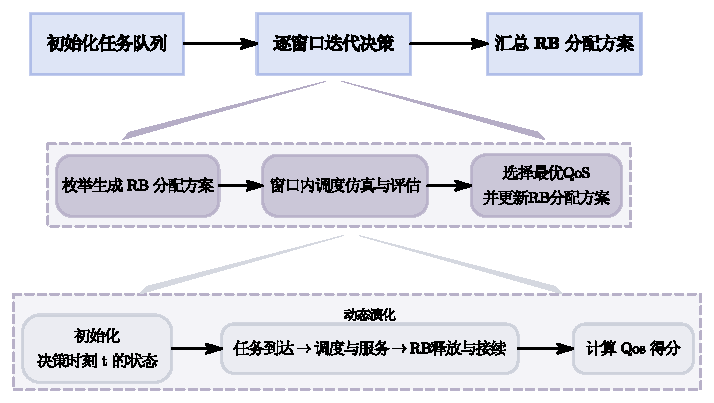
\includegraphics[width=0.85\textwidth]{figures/第二问算法.pdf}
    \caption{问题二MPC动态资源分配与调度算法流程图}
    \label{fig:q2_algorithm_flow}
\end{figure}

\textbf{Step1:初始化}

在仿真开始时刻 $t=0$,初始化所有用户的任务队列为空。

\textbf{Step2:逐窗口迭代决策}

对于每个决策窗口 $w$(对应时间段 $[t, t+100)$,其中 $t = w \times 100$):

\begin{enumerate}
    \item \textbf{生成RB分配方案}:与问题一类似,枚举所有满足约束条件的RB分配方案 $(n_U(t), n_e(t), n_m(t))$,确保资源总量为50,且各切片RB数量分别为10、5、2的倍数。

    \item \textbf{窗口内调度仿真与评估}:对于每个分配方案,进行100ms窗口的详细仿真。仿真从当前系统状态出发,1ms步长推进,动态加入新到达任务,按切片并发能力和“编号靠前优先”原则调度用户,任务完成后立即释放资源并接续新用户。全过程记录任务的到达、服务、完成时刻,计算端到端时延,并据各切片QoS评估函数统计窗口内所有已完成任务的服务质量得分。
    
    \item \textbf{选择最优方案并更新状态}:遍历所有RB分配方案后,我们选择在当前窗口内获得累计QoS总分最高的方案作为本次决策的结果。然后,我们将该最优方案对应的仿真结束时刻($t+100$)的用户队列状态,作为下一个决策窗口的初始状态。
\end{enumerate}

\textbf{Step3:汇总结果}

重复Step2,直到完成所有10个决策窗口($t=0$至$t=900$)的决策。最后,将每个窗口获得的最优QoS得分进行累加,得到整个1000ms内的总服务质量。通过这种方式,我们得到了一系列动态的RB分配决策,以及最终的系统整体性能评估。

\subsection{结果分析}

通过执行上述基于MPC的贪心算法,我们得到了1000ms内的动态资源分配策略,其总服务质量达到了\textbf{352.1029}。

\subsubsection{最优资源分配序列}

算法在10个决策窗口中选择的RB分配序列如下表所示。该序列是在每个窗口选择瞬时最优解(若有多个则选择第一个)的结果。

\begin{table}[H]
\centering
\caption{问题二动态资源分配序列}
\label{tab:q2_decision_sequence}
\begin{tabular}{ccccc}
\hline
\textbf{决策时刻 (ms)} & \textbf{URLLC RB数 ($n_U$)} & \textbf{eMBB RB数 ($n_e$)} & \textbf{mMTC RB数 ($n_m$)} & \textbf{窗口QoS} \\
\hline
0 & 10 & 20 & 20 & 65.490 \\
100 & 10 & 20 & 20 & 40.028 \\
200 & 10 & 20 & 20 & 38.835 \\
300 & 10 & 0 & 40 & 32.800 \\
400 & 20 & 0 & 30 & 31.850 \\
500 & 10 & 0 & 40 & 24.250 \\
600 & 10 & 0 & 40 & 27.100 \\
700 & 20 & 0 & 30 & 32.800 \\
800 & 20 & 0 & 30 & 31.850 \\
900 & 20 & 0 & 30 & 27.100 \\
\hline
\textbf{总计} & - & - & - & \textbf{352.103} \\
\hline
\end{tabular}
\end{table}

在整个仿真周期内,各切片累计获得的QoS分数分别为:URLLC QoS合计\textbf{205.8175},eMBB QoS合计\textbf{46.2854},mMTC QoS合计\textbf{100.0000}。


从资源分配序列(表 \ref{tab:q2_decision_sequence})可以看出,算法展现了良好的动态适应性。在仿真初期(0-300ms),eMBB业务有大量任务到达,算法明智地为其分配了20个RB以快速处理,获得了较高的QoS。在300ms后,eMBB任务队列清空,算法果断地将其RB资源完全回收,转而分配给URLLC和mMTC,以应对后续的URLLC任务并保证mMTC的稳定接入。

综上所述,我们提出的动态资源分配模型与求解算法,能够在时变的信道和任务到达条件下,做出快速有效的决策,实现了系统在整个时间窗口内总服务质量的最优。